
%The salamander is capable of rapidly switching between two locomotion modes: swimming and walking. The muscle movements required for locomotion are executed by the spinal chord and the modal information for which action to execute is delivered by the salamander brain. We attempt to imitate this modal switching behavior of the salamander spinal chord in our own self driving network by feeding in behavioral information to the network. In this case we used two easily distinguishable behavioral modes, follow and direct in contrast to swimming and walking for the salamander. The follow behavioral mode consists of data with our car following another car in front of it, when this car slows down our car should slow down and should follow close behind it. The direct behavioral mode consists of data with the network driving itself on paths at a relatively constant speed.
%For our base network, we used SqueezeNet \cite{iandola2016squeezenet}, since it is a compact network with large receptive fields, and it has shown to be good at regression tasks. The network is slightly modified to allow for 12 channels of input (RGB Color, Left/Right, and current/previous time step). For our MTL network we modified the structure further to support insertion of modal information after the network has done initial processing of visual data.


\section{INTRODUCTION}
\label{sec:intro}


%Learning complex autonomous behaviors like driving, is an ongoing research topic in computer vision and machine learning. Learning based approaches are most effective for dealing with complex or rare scenarios.

Most current research on driving with DNNs has focused on a single driving modality, e.g.\ lane following or obstacle avoidance \cite{bojarski2016end,muller2006off,chen2015deepdriving,DBLP:journals/corr/HuvalWTKSPARMCM15}. We consider these approaches as \textit{Single Task Learning} (STL), as they focus on training to perform an individual task.

%------>In contrast, several methods for other learning problems have learnt multiple tasks simultaneously, in an approach known as Multi Task Learning (M
Multi-task learning (MTL) research has shown that training on side tasks related to the main operation of a deep neural network can enhance its learning capabilities \cite{caruana1998multitask, zhang2012convex}. These side tasks, such as finding the position of sidewalks in the image in addition to driving with lane following, may allow networks to break down image processing into stages and develop specific filters for individual steps in a processing pipeline. In MTL, these side tasks are not used when evaluating networks in inference mode and instead improve performance on the primary task; e.g.\ steering angle prediction.

\begin{figure}[t]
\centering
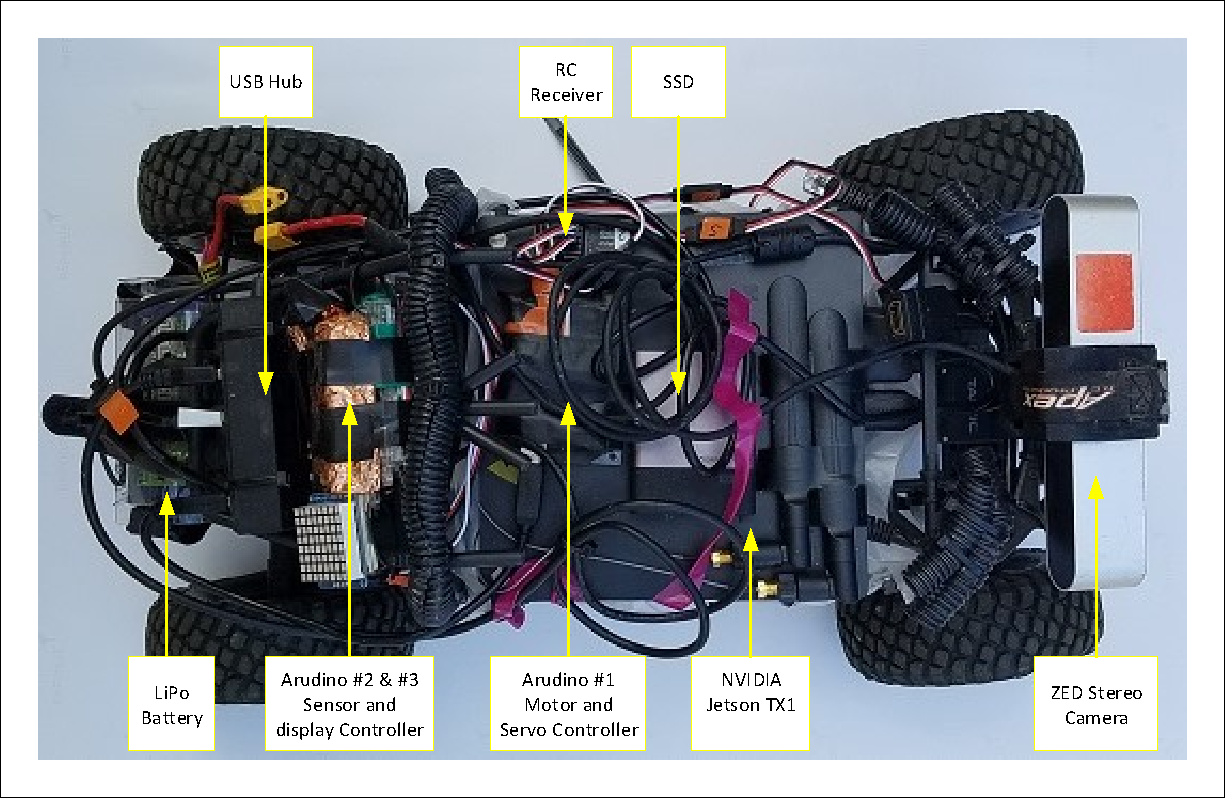
\includegraphics[width=\linewidth,,trim=20 20 20 20,clip]{paper/content/images/car}
\caption{Car Diagram}
\label{fig:cars}
\end{figure}

\afterpage{
\begin{figure*}[!th]
\centering
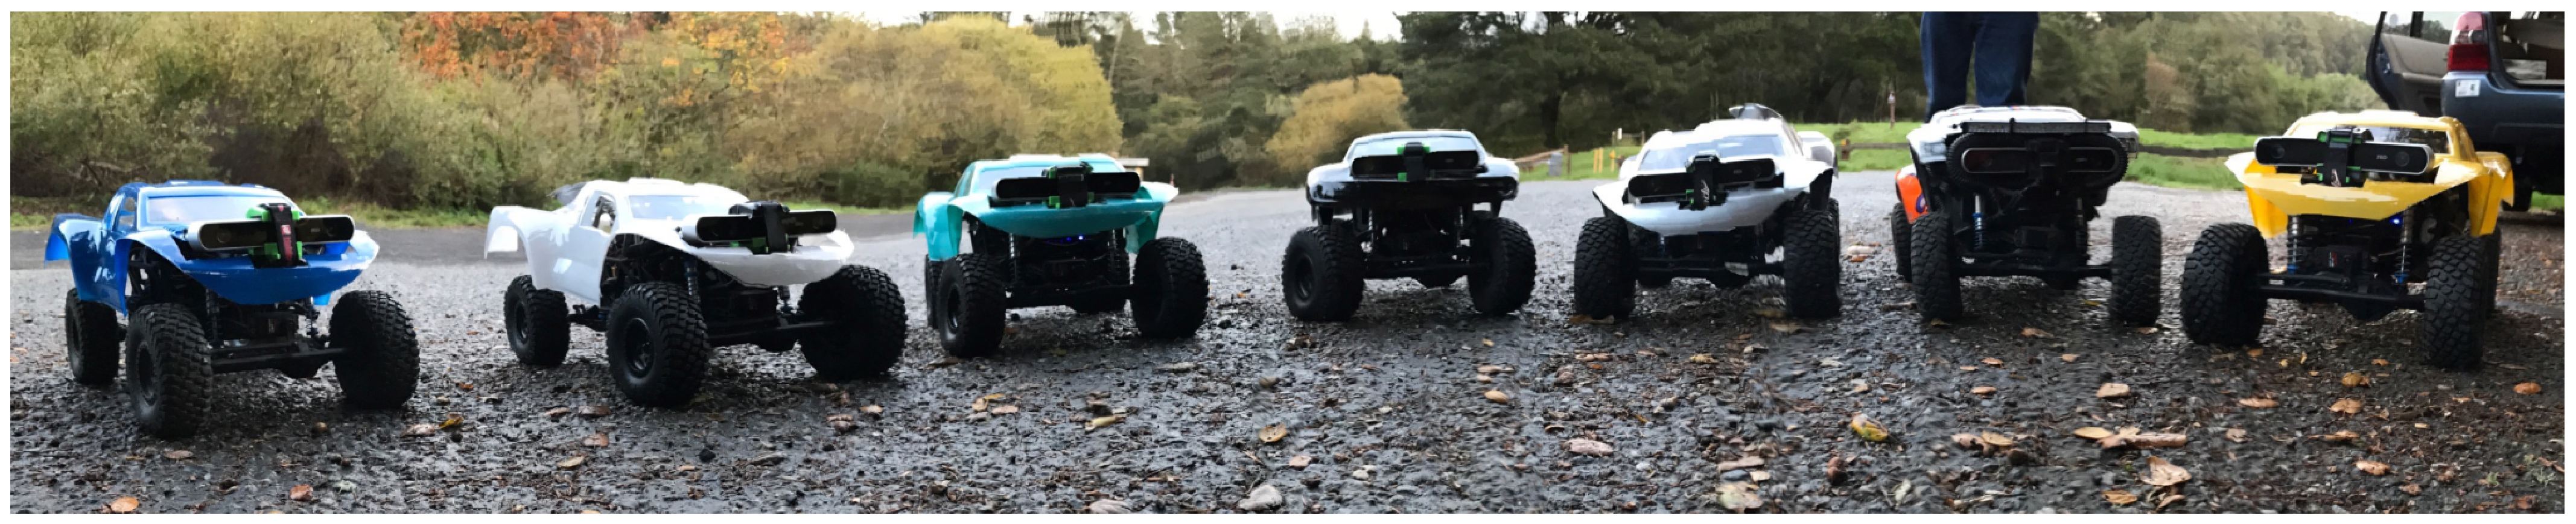
\includegraphics[width=0.9\textwidth]{paper/content/images/fleet}
\caption{Fleet of Model Cars}
\label{fig:fleet}
\end{figure*}
\begin{figure*}[!th]
    \centering
     \begin{subfigure}{0.3\textwidth}
       \centering
       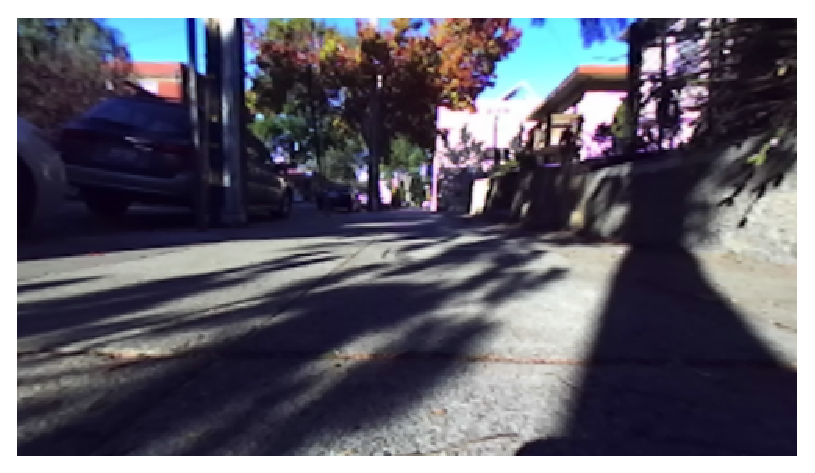
\includegraphics[width=\linewidth]{paper/content/images/daytime}
       \caption{Day Time}
     \end{subfigure}
     \begin{subfigure}{0.3\textwidth}
       \centering
       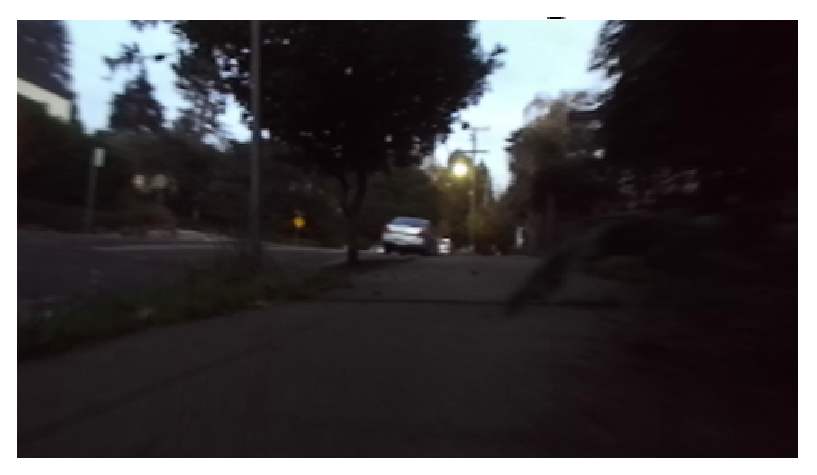
\includegraphics[width=\linewidth]{paper/content/images/evening}
       \caption{Evening}
     \end{subfigure}
     \begin{subfigure}{0.3\textwidth}
       \centering
       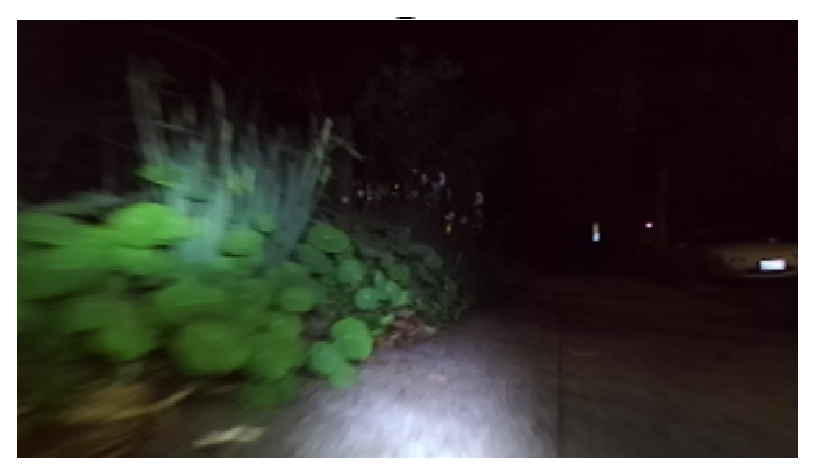
\includegraphics[width=\linewidth]{paper/content/images/night}
       \caption{Night Time}
     \end{subfigure}
        \begin{subfigure}{0.3\textwidth}
       \centering
       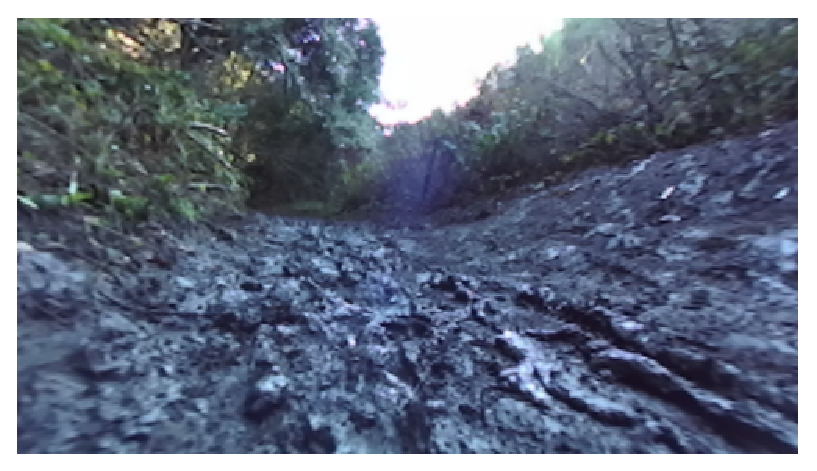
\includegraphics[width=\linewidth]{paper/content/images/muddy}
       \caption{Muddy Area}
    \end{subfigure}
    \begin{subfigure}{0.3\textwidth}
       \centering
       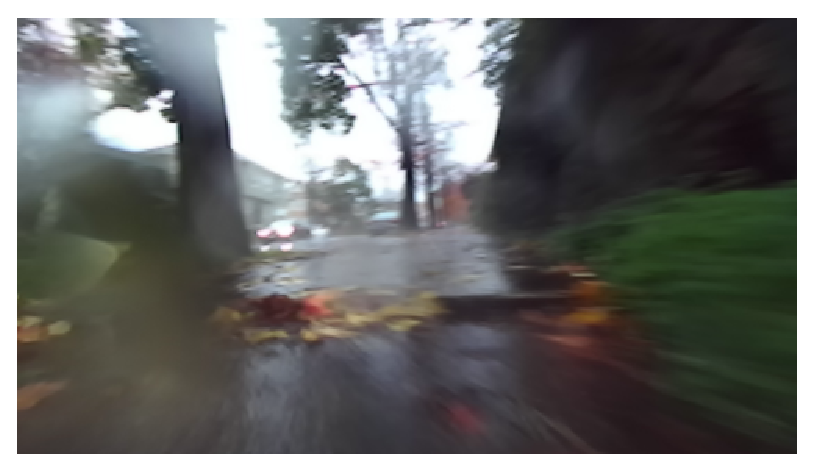
\includegraphics[width=\linewidth]{paper/content/images/rainy}
       \caption{Rainy Area}
    \end{subfigure}
    \begin{subfigure}{0.3\textwidth}
       \centering
       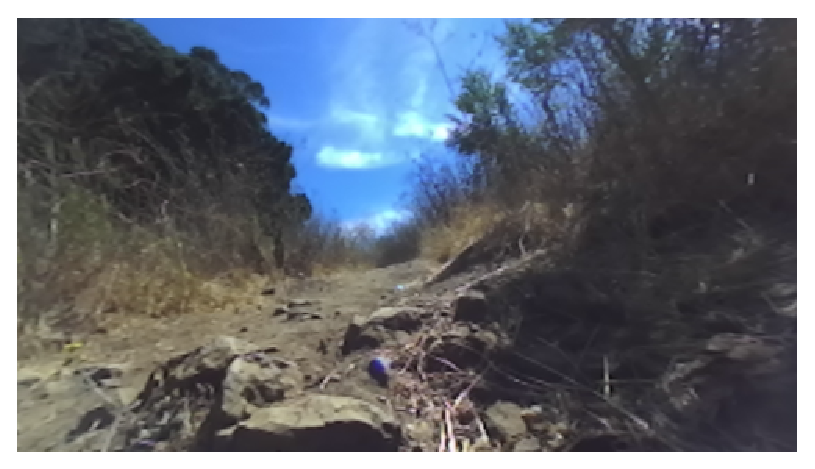
\includegraphics[width=\linewidth]{paper/content/images/bumpy}
       \caption{Bumpy Area}
    \end{subfigure}
    \caption{Diverse Conditions in Dataset}
    \label{fig:diverse}
\end{figure*}

\begin{figure*}[!th]
    \centering
    \begin{subfigure}{0.3\textwidth}
       \centering
       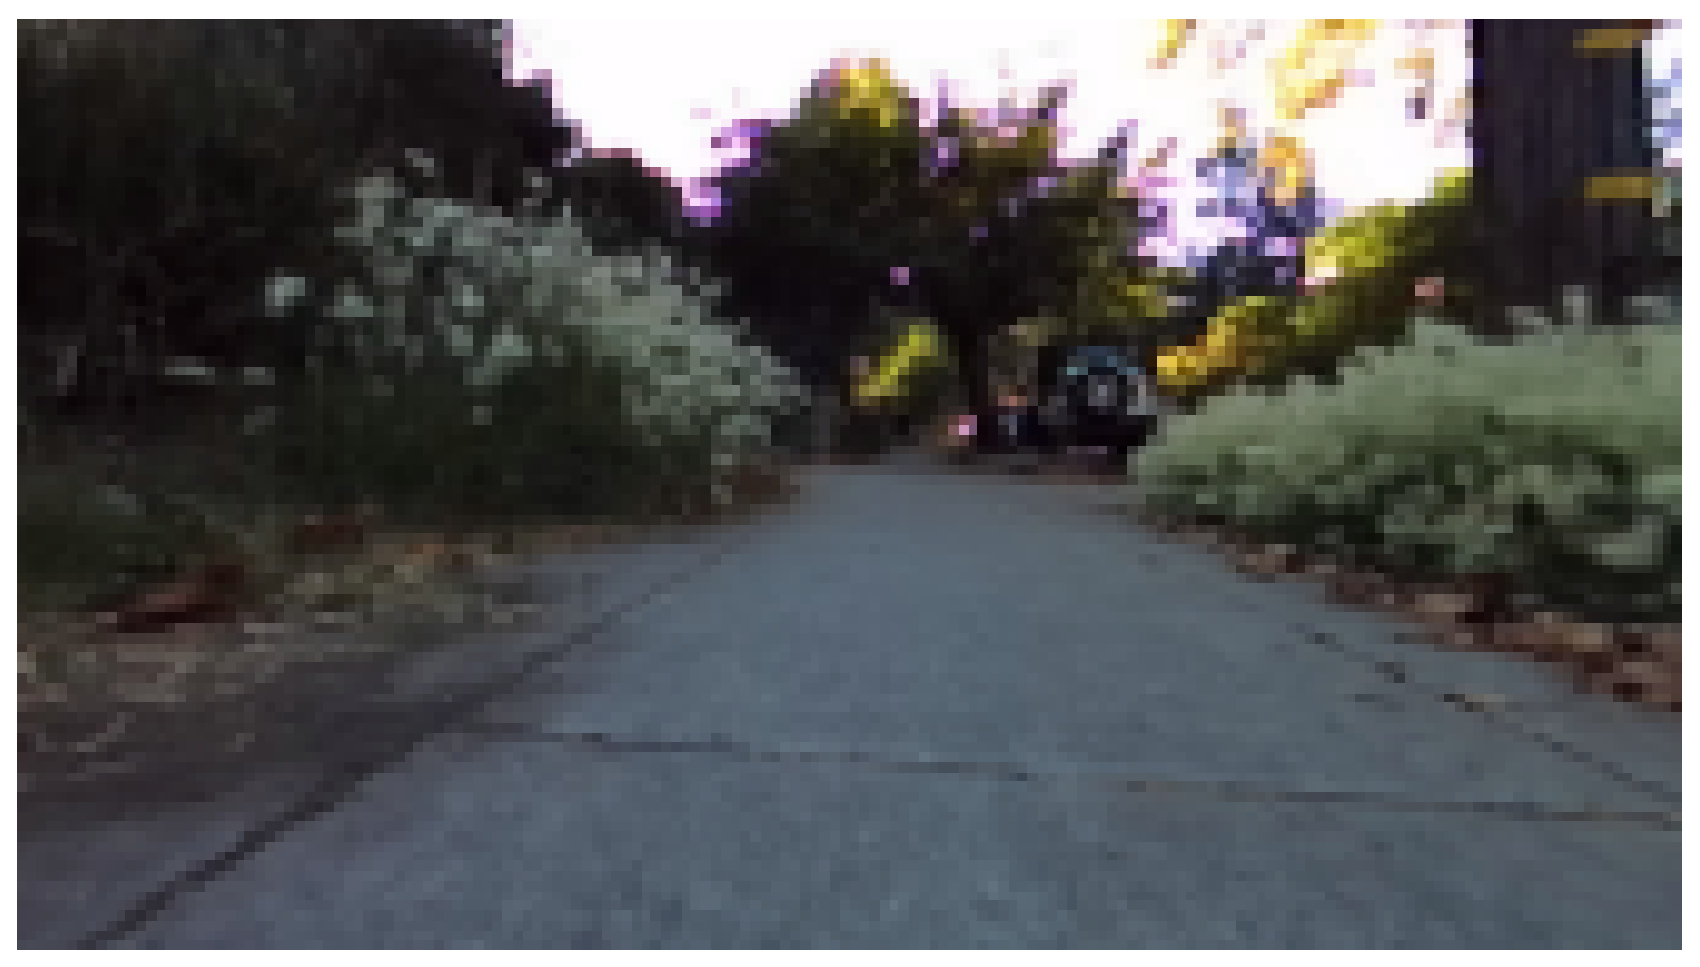
\includegraphics[width=\linewidth]{paper/content/images/directexample}
       \caption{Direct Mode}
       \label{fig1:direct}
    \end{subfigure}
    \begin{subfigure}{0.3\textwidth}
       \centering
       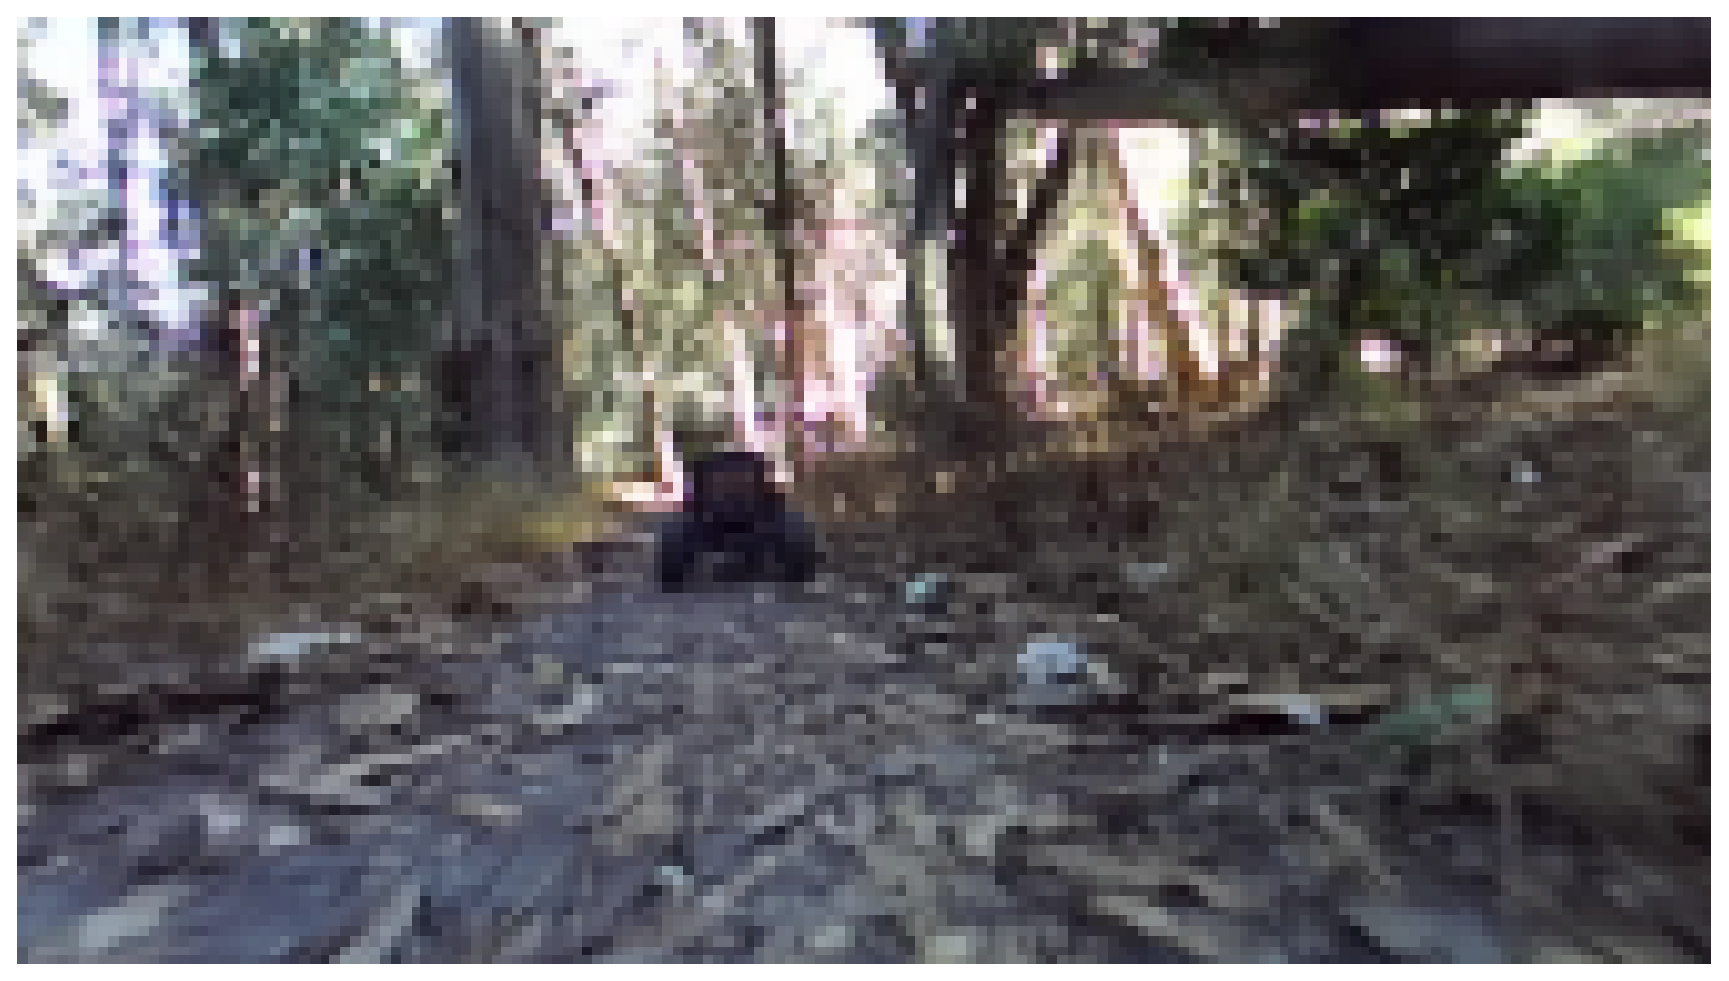
\includegraphics[width=\linewidth]{paper/content/images/followexample}
       \caption{Follow Mode}
       \label{fig1:follow}
    \end{subfigure}
    \begin{subfigure}{0.3\textwidth}
       \centering
       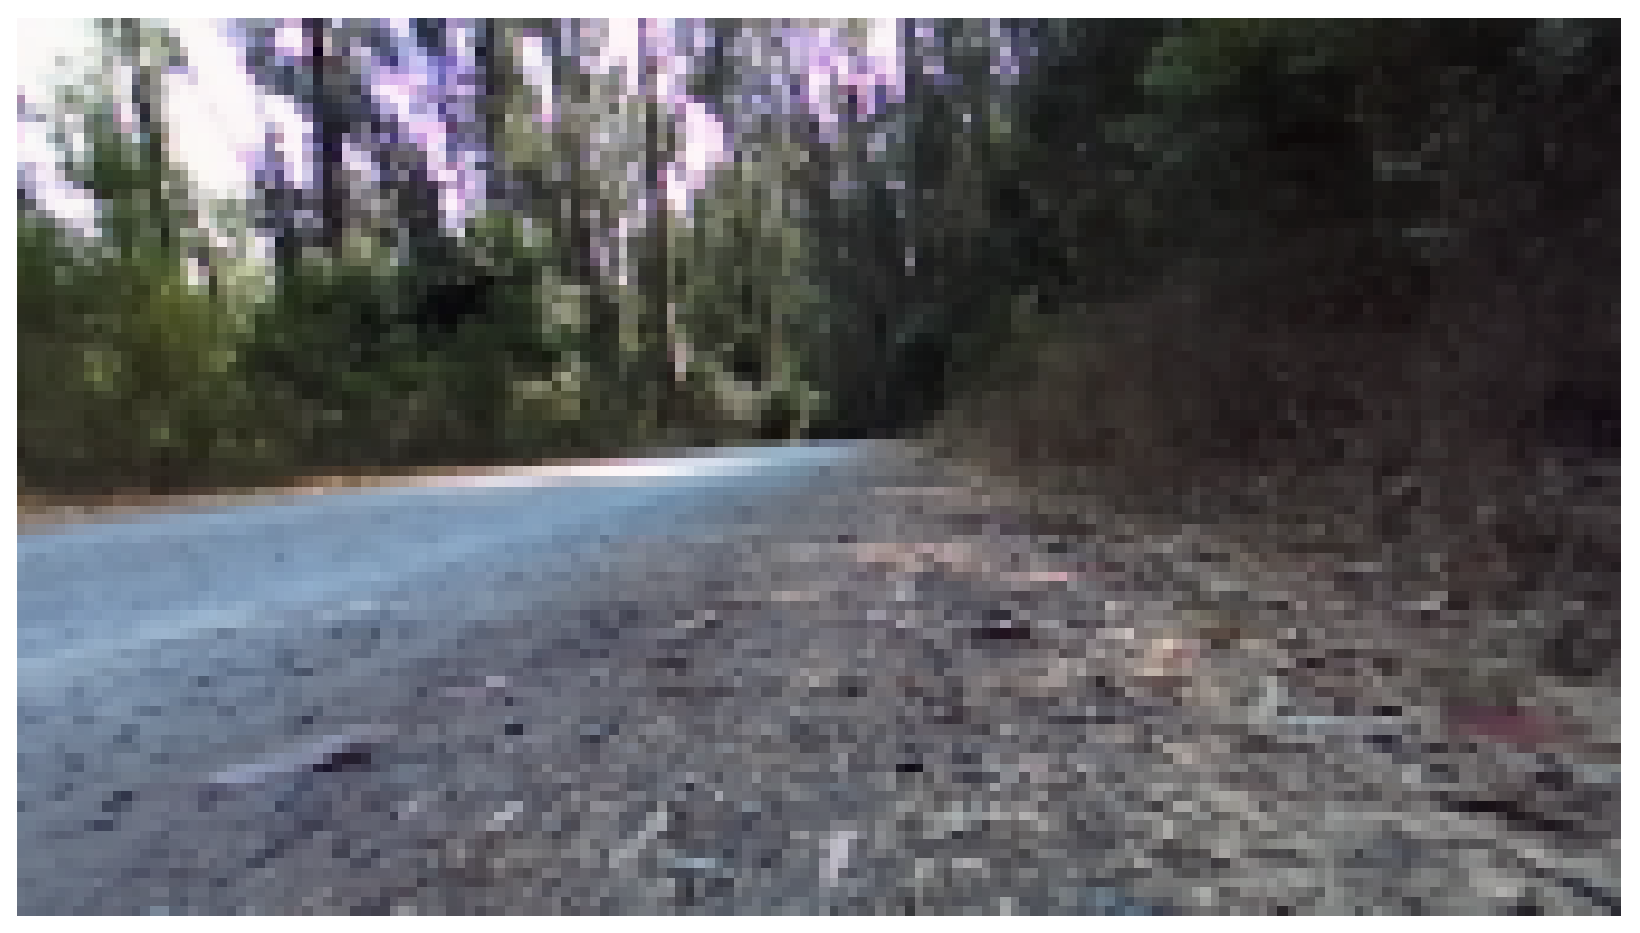
\includegraphics[width=\linewidth]{paper/content/images/furtiveexample}
       \caption{Furtive Mode}
       \label{fig1:furtive}
    \end{subfigure}
    \caption{Behavioral Mode Sample Data from Car's Point of View}
    \label{fig1:behavioralmodes}
\end{figure*}
}

Additional research is being conducted on multi-modal learning, a method in which networks are trained on several distinct modes of operation, all of which are used during inference.
For example, a network which has the single task of transcribing audio to text may be given a side task of sentiment analysis to improve performance in the transcribing task \cite{6639012}. This is a multi-task learning network as the side-task of sentiment analysis is not needed during inference and is merely used to improve performance on a different task. If instead the network is given the task of transcribing text in two modes: one for audio, and the other for video recordings \cite{ngiam2011multimodal}. This is an example of multi-modal learning as there are multiple modes of running the network either of which can be used during evaluation.

Work on multi-modal learning has predominantly been focused in fields other than robotics or locomotion; e.g.\ speech recognition with audio and video \cite{ngiam2011multimodal, 6639012}. Within these works, it is common for DNNs to be given input that could correspond to any or multiple modes of operation. 

In the context of performing multiple tasks multi-modal networks have significantly fewer parameters when compared to systems with multiple networks, as multiple related tasks can be completed by a single network rather than multiple networks. Smaller network sizes are desirable as they allow for fast over the air model updates in self driving cars, and deployment on Field Programmable Gate Arrays (FPGA) \cite{DBLP:journals/corr/IandolaMAHDK16}.
% The MTL side tasks consist of additional motor and steering values inferred by the network, which are not used for actuation on the vehicles at the time of evaluation.
In this paper, we propose a new method for combining multi-modal learning with MTL for autonomous driving.
In this method, the MTL side tasks consist of additional motor and steering values inferred by the network, which are not used for actuation on the vehicles at time of evaluation. These side-tasks are akin to sentiment analysis in the prior example.
Additionally, we introduce multiple distinct driving behaviors, or \textit{behavioral modes}, in which the model car can operate.
These behaviors constitute the modes of evaluation for multi-modal learning, akin to audio and video in the previous example.
The behavioral modes are given to the network as a privileged secondary input, allowing for separate driving behaviors to form within a single network.

% In this approach, side tasks consist of separate driving behaviors which are all used during inference. Additionally, the current mode of operation is given to the network as a secondary input, allowing for separate driving behaviors to form within a single network.
We denote our multi-modal MTL networks as \textit{MultiNets} in contrast to the MTL networks trained in a single behavioral mode. We show that in addition to having a size advantage over a simple MTL approach, MultiNets exceed the performance of multiple MTL networks on the same tasks in evaluation on a validation dataset as well as in on-the-road experiments.

The concurrent work of \cite{intel_paper} investigates a multi-modal approach with multiple sub-networks for each mode and provides a mathematical justification for the insertion of privileged modal data. Our approach differs in that a single general and scalable network is used to infer an arbitrary number of behavioral modalities using a novel logical modal switch in the processing stream of the network.

This paper is organized as follows.
Section \ref{sec:dataset} covers the methods of collection of our dataset, as well as detailing the robotic cars used in the work.
Section \ref{sec:approach} describes the specific innovations of MultiNets, as well as introducing our own deep convolutional neural network, \textit{Z2Color}, used for training and running experiments.
Section \ref{sec:experiments} covers the experiments conducted through evaluation of network validation loss for multiple and individual behavioral modes, as well as evaluation in on-the-road tests.
Finally, Section \ref{sec:conclusion} summarizes the major contributions of this paper and suggests areas for future work.
% In the self driving case, researchers have also shown how DNNs can be trained to predict and distinguish between separate driving modalities such as turning or stopping \cite{xu2016end}.


